\section{Logical view}

Som beskrevet i view beskrivelser på forrige side består logical viewet af designoverview-, sekvens-, statemachines og klassediagrammer. Til at lave diagrammerne anvendes applikationsmodellen.

\subsection{Applikationsmodel}
Applikationsmodellen anvendes til at udvikle diagrammerne tilhørende logical view. Med applikationsmodellen tages der udgangspunkt i use cases beskrevet i kravspecifikationen og domain modellen, se figur \ref{fig:domain_model}.
  
Ud fra domain modellen identificeres de overordnede klasser der skal bruges til de forskellige use cases. Når de overordnede klasser er identificeret beskrives hvordan de kommunikerer via desginoverview og sekvensdiagrammer. Herefter laves statemachines med de fundne klasser og til sidst udarbejdes klassediagrammer.


\subsection{Use case 1 - Start drone}

Bruger tænder dronen ved at tilslutter batteri. Main controller samt 3G/GPS initialiseres og nuværende GPS position opdateres.
Herefter oprettes forbindelse mellem drone og webapplikation. Når forbindelsen er på plads sendes handshake og information om nuværende GPS position fra dronen til webapplikation. Dronen er nu klar til at modtage flyveopsætning fra server.

\vspace{-5pt}
%kommentar
\begin{figure}[H]
	\centering
	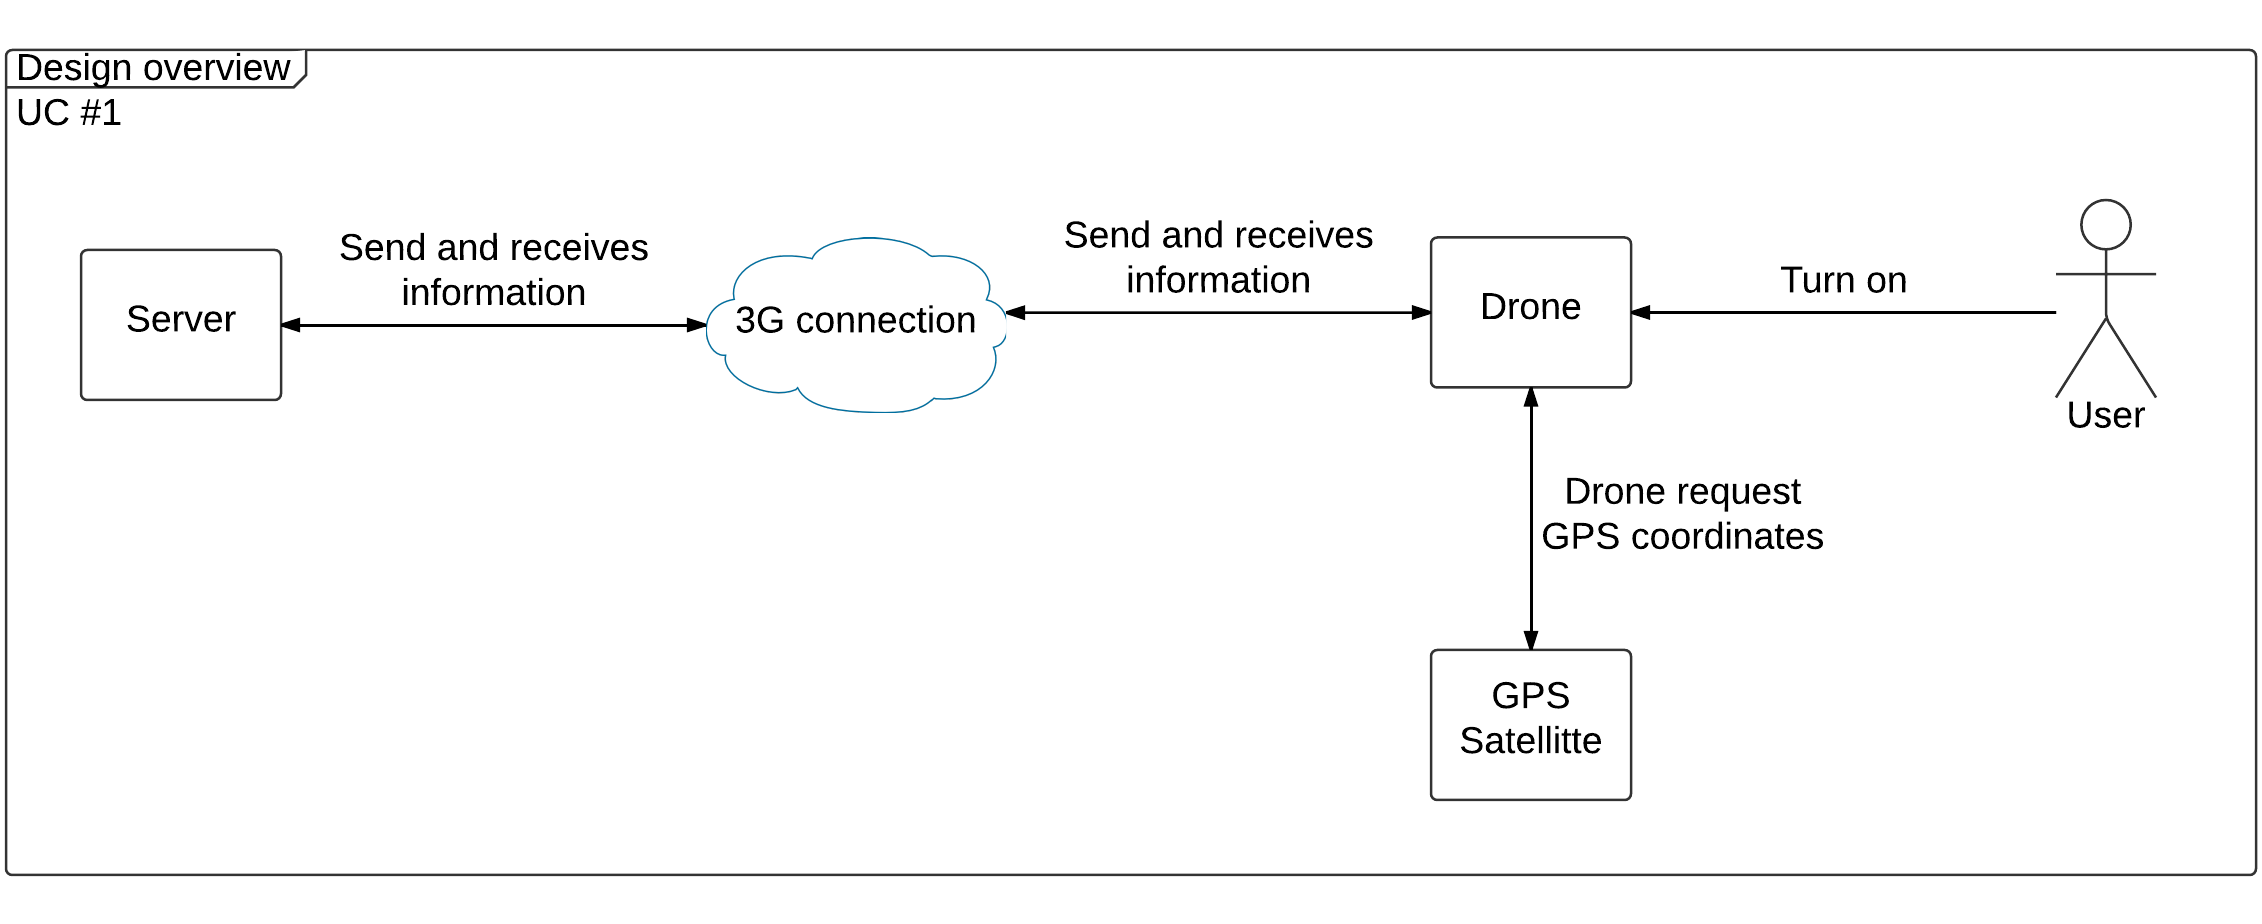
\includegraphics[width=1\textwidth]{Billeder/design_overview/design_overview_UC1.png}
	\vspace{-1cm}
	\caption{Design overview \#UC1 - Start drone}
	\label{fig:design_overview_UC1}
\end{figure}


\newpage

På dette sekvensdiagram vises det hvilke klasser der indgår og bruges i UC1. Af sekvensdiagrammet fremgår det at sekvensen først startes når bruger tilslutter batteri og tænder dronen 

\vspace{-5pt}
%kommentar
\begin{figure}[H]
	\centering
	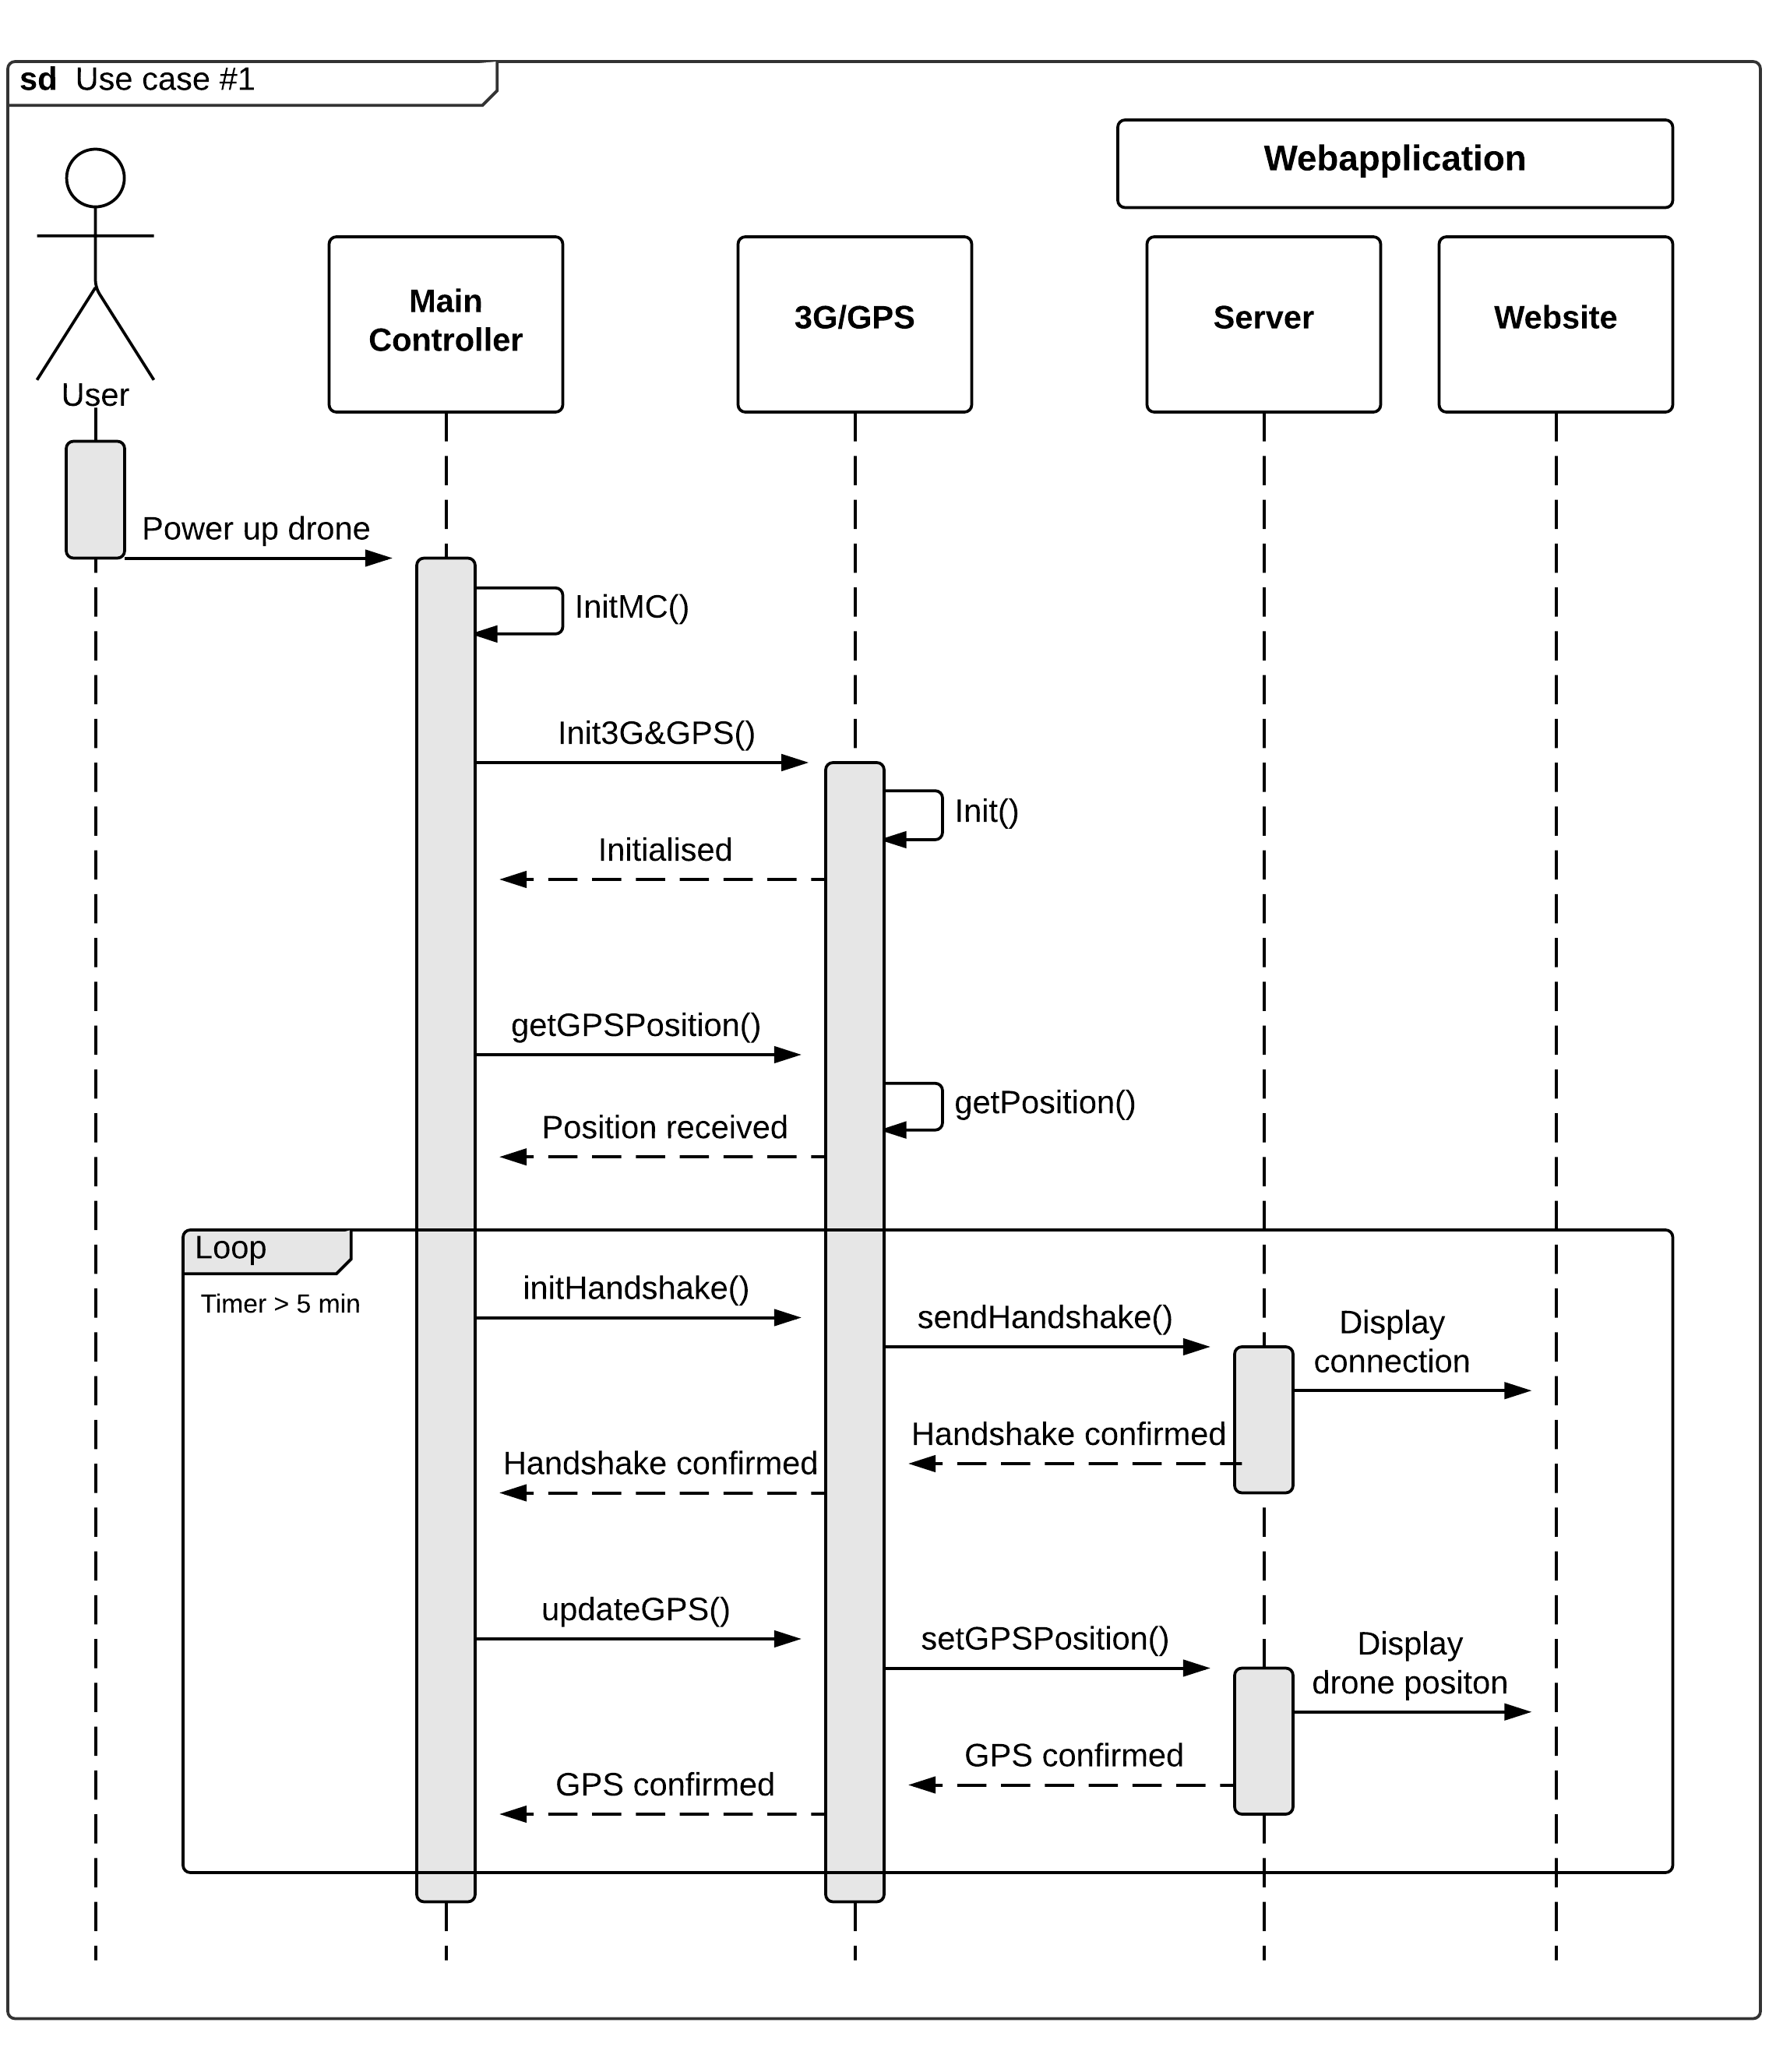
\includegraphics[width=1\textwidth]{Billeder/sekvens/sekvens_UC1.png}
	\vspace{-1cm}
	\caption{Sekvens diagram \#UC1 - Start drone}
	\label{fig:Sekvens diagram_UC1}
\end{figure}

\newpage

På statemachine diagrammet vises de forskellige stadier i use case 1, samt flowet imellem dem.
\vspace{-5pt}
%kommentar
\begin{figure}[H]
	\centering
	\includegraphics[width=1\textwidth]{Billeder/statemachine/state_UC1.png}
	\vspace{-1cm}
	\caption{Statemachine \#UC1 - Start drone}
	\label{fig:Statemachine_UC1}
\end{figure}

